% 2008 年福建卷理科第 12 题：已知 y=f(x)、y=g(x) 的导函数图象（f' 递减、g' 递增，
%   在 x=x0 处相交），选 f、g 的图象可能的一组。
% 来源 PDF：gaokaomath-src/普通高考/2008/2008福建理.pdf
% SHA-256：516e8ac8e113868afa9bc4af4724c3b43f22a1f7fecc830a7f3400b8d973d452
% 原页：2008福建理.pdf 第 1 页（A3 三栏）第 2 栏，书页码 441。
% 绘制依据：f' 递减、g' 递增且在 x0 相交，故 f-g 在 x0 取极大；四组候图中只有 (C)
%   满足两曲线在 x0 处相切且 f 在 g 下方，与原页排成 2×2。
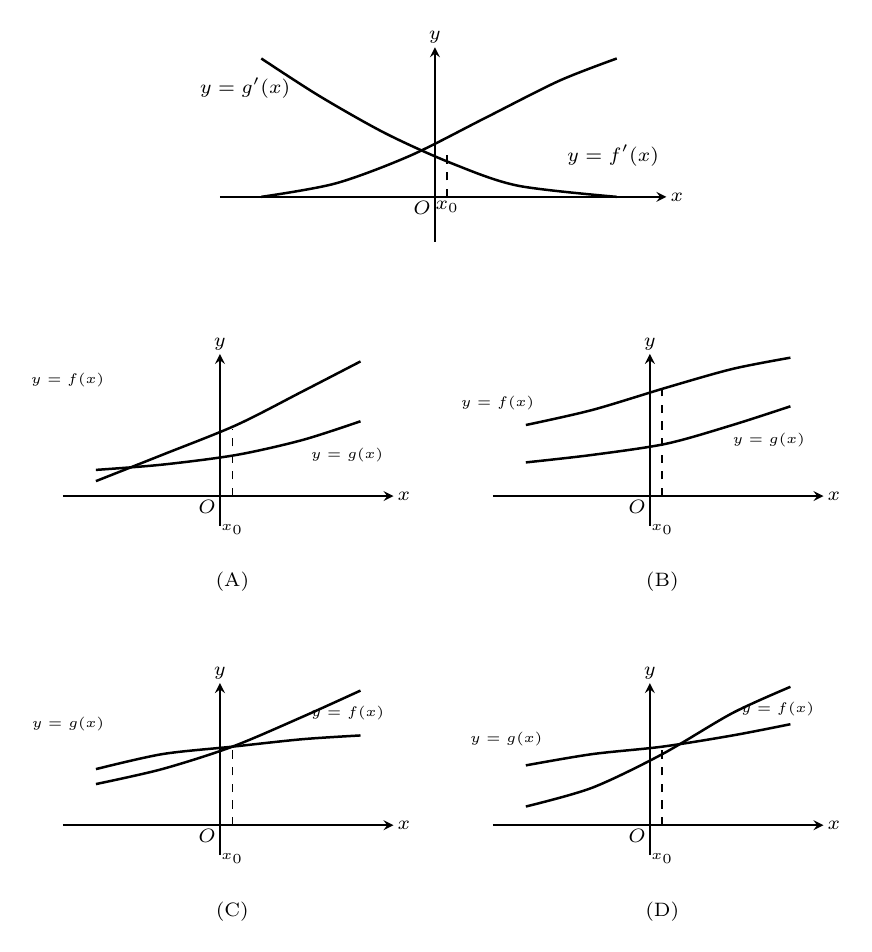
\begin{tikzpicture}[x=1.05cm, y=0.95cm, semithick, font=\scriptsize,
  every node/.style={inner sep=1.2pt}]

  % ---- 题干：导函数图象 ----
  \begin{scope}[shift={(0,0)}]
    \draw[->,>=stealth] (-2.6,0) -- (2.8,0) node[right] {$x$};
    \draw[->,>=stealth] (0,-0.6) -- (0,2.0) node[above] {$y$};
    \node[below left] at (0,0) {$O$};
    \draw[line width=0.9pt, smooth, samples=90]
      plot coordinates {(-2.1,1.85) (-1.4,1.35) (-0.6,0.85) (0.2,0.45) (1.0,0.15) (2.2,0.0)};
    \draw[line width=0.9pt, smooth, samples=90]
      plot coordinates {(-2.1,0.0) (-1.2,0.18) (-0.3,0.55) (0.6,1.05) (1.5,1.55) (2.2,1.85)};
    \draw[dashed] (0.15,0) -- (0.15,0.62);
    \node[below] at (0.15,0) {$x_0$};
    \node[right] at (1.55,0.55) {$y=f'(x)$};
    \node[left] at (-1.70,1.45) {$y=g'(x)$};
  \end{scope}

  % ---- (A) ----
  \begin{scope}[shift={(-2.6,-4.0)}]
    \draw[->,>=stealth] (-1.9,0) -- (2.1,0) node[right] {$x$};
    \draw[->,>=stealth] (0,-0.4) -- (0,1.9) node[above] {$y$};
    \node[below left] at (0,0) {$O$};
    \draw[line width=0.9pt, smooth, samples=90]
      plot coordinates {(-1.5,0.2) (-0.7,0.55) (0.2,0.95) (1.0,1.4) (1.7,1.8)};
    \draw[line width=0.9pt, smooth, samples=90]
      plot coordinates {(-1.5,0.35) (-0.7,0.42) (0.2,0.55) (1.0,0.75) (1.7,1.0)};
    \draw[dashed] (0.15,0) -- (0.15,0.9);
    \node at (0.15,-0.45) {\tiny $x_0$};
    \node[left] at (-1.35,1.55) {\tiny $y=f(x)$};
    \node[right] at (1.05,0.55) {\tiny $y=g(x)$};
    \node at (0.15,-1.15) {(A)};
  \end{scope}

  % ---- (B) ----
  \begin{scope}[shift={(2.6,-4.0)}]
    \draw[->,>=stealth] (-1.9,0) -- (2.1,0) node[right] {$x$};
    \draw[->,>=stealth] (0,-0.4) -- (0,1.9) node[above] {$y$};
    \node[below left] at (0,0) {$O$};
    \draw[line width=0.9pt, smooth, samples=90]
      plot coordinates {(-1.5,0.95) (-0.7,1.15) (0.2,1.45) (1.0,1.7) (1.7,1.85)};
    \draw[line width=0.9pt, smooth, samples=90]
      plot coordinates {(-1.5,0.45) (-0.7,0.55) (0.2,0.7) (1.0,0.95) (1.7,1.2)};
    \draw[dashed] (0.15,0) -- (0.15,1.45);
    \node at (0.15,-0.45) {\tiny $x_0$};
    \node[left] at (-1.35,1.25) {\tiny $y=f(x)$};
    \node[right] at (0.95,0.75) {\tiny $y=g(x)$};
    \node at (0.15,-1.15) {(B)};
  \end{scope}

  % ---- (C) ----
  \begin{scope}[shift={(-2.6,-8.4)}]
    \draw[->,>=stealth] (-1.9,0) -- (2.1,0) node[right] {$x$};
    \draw[->,>=stealth] (0,-0.4) -- (0,1.9) node[above] {$y$};
    \node[below left] at (0,0) {$O$};
    \draw[line width=0.9pt, smooth, samples=90]
      plot coordinates {(-1.5,0.55) (-0.7,0.75) (0.15,1.05) (1.0,1.45) (1.7,1.8)};
    \draw[line width=0.9pt, smooth, samples=90]
      plot coordinates {(-1.5,0.75) (-0.7,0.95) (0.15,1.05) (1.0,1.15) (1.7,1.2)};
    \draw[dashed] (0.15,0) -- (0.15,1.05);
    \node at (0.15,-0.45) {\tiny $x_0$};
    \node[left] at (-1.35,1.35) {\tiny $y=g(x)$};
    \node[right] at (1.05,1.5) {\tiny $y=f(x)$};
    \node at (0.15,-1.15) {(C)};
  \end{scope}

  % ---- (D) ----
  \begin{scope}[shift={(2.6,-8.4)}]
    \draw[->,>=stealth] (-1.9,0) -- (2.1,0) node[right] {$x$};
    \draw[->,>=stealth] (0,-0.4) -- (0,1.9) node[above] {$y$};
    \node[below left] at (0,0) {$O$};
    \draw[line width=0.9pt, smooth, samples=90]
      plot coordinates {(-1.5,0.25) (-0.7,0.5) (0.15,0.95) (1.0,1.5) (1.7,1.85)};
    \draw[line width=0.9pt, smooth, samples=90]
      plot coordinates {(-1.5,0.8) (-0.7,0.95) (0.15,1.05) (1.0,1.2) (1.7,1.35)};
    \draw[dashed] (0.15,0) -- (0.15,1.05);
    \node at (0.15,-0.45) {\tiny $x_0$};
    \node[left] at (-1.25,1.15) {\tiny $y=g(x)$};
    \node[right] at (1.05,1.55) {\tiny $y=f(x)$};
    \node at (0.15,-1.15) {(D)};
  \end{scope}
\end{tikzpicture}
